\documentclass{report}

\usepackage[utf8]{inputenc}
\usepackage{titling}
\usepackage{natbib}
\usepackage{graphicx}
\usepackage{enumitem}
\usepackage{hyperref}

\usepackage{listings}
\usepackage{color}


\definecolor{dkgreen}{rgb}{0,0.6,0}
\definecolor{gray}{rgb}{0.5,0.5,0.5}
\definecolor{mauve}{rgb}{0.58,0,0.82}

\lstset{frame=tb,
  language=C,
  aboveskip=3mm,
  belowskip=3mm,
  showstringspaces=false,
  columns=flexible,
  basicstyle={\small\ttfamily},
  numbers=none,
  numberstyle=\tiny\color{gray},
  keywordstyle=\color{blue},
  commentstyle=\color{dkgreen},
  stringstyle=\color{mauve},
  breaklines=true,
  breakatwhitespace=true,
  tabsize=2
}
\lstMakeShortInline[columns=fixed]|

%\usepackage[parfill]{parskip}

% Destroy the Annoying Margins.
\hoffset 0pt
\voffset 0pt
\headsep 0pt
\headheight 0pt
\oddsidemargin 0in 
\evensidemargin 0in 
\textwidth 6.5in \textheight 9in

\title{ReverseEngineering}
\begin{document}

\begin{titlepage}
    \vspace*{-2cm}
    \begin{center}
        {\Huge \bfseries CST Training \par}
        \vspace{1cm}
        {\large \bfseries Reverse Engineering  \par}

    \end{center}
    \begin{center}
        \vspace{3cm}
        
\includegraphics[scale=.6]{usna-seal.png}
        \vspace{1cm}
    \end{center}
    

  
    \begin{center}
        {\LARGE\bfseries United States Naval Academy \break \par}
        {\Large\bfseries Cyber Security Team \par}

    \end{center}
  
    \vspace{3.0cm}
   


\end{titlepage}


\newpage

\tableofcontents

\newpage

\chapter{Lesson Plan}
 
\section{Introduction}
In this lesson we will go over how to go about reverse engineering a binary.
 
\section{Objectives}
 \begin{enumerate}
    \item Be able to read x86 assembly language and be able to imagine the C code that went into writing it.
    \item Learn what tools are used when reversing a binary and how to use each of them.
    \item Know how to patch a binary so that you can edit out things.
    \item Know how to get unpack a binary
    \item know how to de-obfuscation
    \item Learn about Windows debugging 
    \item Other assembly Languages
\end{enumerate}

\section{Disclaimer}
This chapter is assuming that you already know how to code in x86 assembly.

\newpage

\chapter{Assembly Crash Course}

\section{What is Assembly}
Assembly a low level language that is almost the machine code that the computer understands.  When you write out any program, before it gets run it must be converted into Assembly.  This is either done by the user (such as running gcc to compile a c program) or by the program itself (such as java compiling something into java byte code).  The compiler turns the code the user wrote into op codes.  These op codes are literally 1's and 0's which are more commonly viewed in hexadecimal.  These hexadecimal numbers directly correspond to assembly instructions.  

\section{Parts of Memory}
\begin{verbatim}

higher address
0xffffffff --> .----------------.
               |    reserved    |  <-- command line args
               +----------------+      environment variables
               |                |
               |     stack      |  <-- user stack, function frames
               |       |        |
               :       |        :
               '       v        '
                                   <-- mapped data
               .       ^        .
               :       |        :
               |       |        |
               |     heap       |  <-- user heap, dynamic memory
               +----------------+
               |      bss       |  <-- global memory 
               +----------------+
               |     text       |  <-- code segments
0x00000000 --> '----------------'
lower address

From Doctor Aviv notes
\end{verbatim}
In memory the stack is where functions store their information.  We will talk a lot about the stack.  The heap is where memory that is allocated is pointed to.
It is not necessary to know what each part of memory is for other than the stack and the heap but if you do want to know more.
\url{https://en.wikipedia.org/wiki/Data_segment#Program_memory}

\section{The Stack}
Computers are not magic.  They do not simply know things nor can they simply remember things.  Any and every piece of information (even if it is currently using it) gets stored somewhere.  This may seem like a pretty obvious statement but then where does a computer store information.  Everything gets stored in either Memory or in a register.  So what is this "Stack" that I keep hearing all the cool kids on the school yard talking about?  The Stack is not some new drug, it is part of the computers memory (RAM or random access memory).  The stack is a chunk of memory that is allocated specifically at the beginning of each function for use for that function.  During this function, that chuck of the stack is currently active and can be used to store information into.  After that function ends that space in memory is deallocated and is open for future use.  The stack is probably one of the most talked about part of reversing and exploiting binaries.

\section{Registers}
Depending on if you are looking at 32 bits vs 64 bits there are different registers.  But all of them are broken down in a similar fashion:
\begin{verbatim}
                                 32 bits (eax)
|------------16 bits------------------|-------------16 bits (ax)-------------|
                                                       8 bits      8 bits 
.----------------------------------------------------------------------------.
|_____________________________________|______________|___(ah)___|_____(al)___|
\end{verbatim}
In a 32 bit operating system every register is 32 bits.  There are 10 different registers that are all used for different things: EAX, EBX, ECX, EDX, ESI, EDI, EBP, ESP, and EIP.  The full register is 32 bits so EAX is 32 bits (E for extended from the original 16 bit registers).  Then each register can be broken down further, the lower 16 bits are AX (or BX or CX depending on which register you are looking at).  Then AX can be broken down again into the 8 bit AH and AL registers (high and low).  Here is what each of them are generally used for:

EAX: Called the accumulator register is typically used to store return values from functions.\newline

EBX: This register is generally used to point to the base of an array.\newline

ECX: This register is typically used as a counter (e.g. loops, iterating through an array etc).\newline

EDX: This is mostly used as a supporting register. It is used a lot in multiplication and when 64 bit return values are returned in EDX:EAX in the code generated by 32 bit compilers.\newline

ESI: The source index for string operations.\newline

EDI: The destination index for string operations.\newline

EBP (Base pointer): Points to the base (i.e. bottom) of the current function’s stack frame.\newline

ESP (Stack pointer): Points to the current position (i.e. top) of the current function’s stack frame.\newline

EIP: This register points to the address of the next instruction.\newline

EFlags: This is a special register that most people do not directly talk about.  It holds the values of what are called FLAGS.  There are 17 necessary flags and each flag holds one to two bits.  We will not cover what all the flags are or what they are all used for but just know that they are most commonly used when the computer compares two registers and will set a flag to determine if they are equal, less than, greater than, etc.  \hyperref[ref:2]{\textbf{References: (a)}}   

\section{Basic Instructions}
There are about 20 instructions that you should simple know.  If you ever find an instruction outside of these then you will probably have to look it up but it will also be likely unimportant to you.  There are two major types of syntax to display x86/64 assembly instructions, intel and AT\&T.  We will use intel but it is good to understand how both look in case you do not get to choose the style that is provided to you.  In intel format, registers in instructions are ordered such that from rigth to left is destination, source.\newline

I strongly recommend having a reference guide to x86 instructions until a familiarity has been made.  \url{https://en.wikibooks.org/wiki/X86_Assembly/X86_Instructions} Has a well written examples of all of these instructions as you might need them.\newline


Format of operations: \newline
Most instructions take either 1 or 2 operands.  The instructions that take two operands, in Intel syntax, are layed out as: ``destination, source". The destination can either be a register or memory address.  The source can either be a register, memory address, or a constant.\newline


NOTES::
braces means do the math and follow the pointer, then the PTR means move the whole 4 byte thing into it.\newline

add - adds src to dest (ex. add eax, ebx adds the contents of ebx to eax)\newline

sub - subtracts dest from src (ex. sub ebp, 0x20 subtracts hex 20 (32 decimal) from ebp)\newline

imul - multiplies dest and src and stores in the first argument. (ex. imul eax, ebx multiplies the contents of eax and ebx together and stores it in eax. There are many different variants of mul/imul and if you come across these then you can easily lookup how they work). \newline

inc - Takes 1 operand (register or memory address) and increments it by 1.\newline

dec - Takes 1 operand (register or memory address) and decrements it by 1.\newline

mov (variants) - Moves (or copies) value from src to dest.  There are other types of mov such as movzx which does the same as mov but also zero extends the remaining digits in the register.\newline

cmp - compare compares operand 1 and 2 and will set flags accordingly.  This is generally used before a jump so that you may for example jump if less than. \hyperref[ref:2]{\textbf{References: (a)}} \newline

test - takes two values and does \textbf{all} the conditional testing and stores all the answers in the flags. test is similar to cmp, the difference is that test does even more tests.  Often times you will see ``test al, al" which is used to see if al is null.\newline

jmp (variants) - jmp takes 1 operand, an address or relative location, and jumps to it. There are other jmp such as: jle (jump less than or equal), jl (jump if less than), je (jump if equal), etc. These will jump or not jump based on which flags are set.  This is why a jump is usually done after a cmp or test. \hyperref[ref:2]{\textbf{References: (b)}} \newline

call - The call mnemonic pushes the eip to the stack and does a jump command to the start of the address of the function that it is about to call so that the computer may start to run that function. \newline

lea - Load effective Address of the sources memory address into destination This means that it follows the pointer to its values. so if we see ``lea eax, [ebp-0x1b]" this means that eax because the value that ebp-x01b is pointing to. lea is a move with math the you do with pointers.\newline

shifting (shr, shl, sar, sal, ror, rol) - Bitwise shifting of registers by the given amount.\newline

xor - xors src with dest\newline

nop - nop stands for No Operation. Nothing is done on a nop, eip is merely incremented to the next instruction.  This be used to keep the alignment of the stack.\newline

push - copies the contents of the given register onto the stack and decrements esp by 1 (remember the stack grows down).\newline

pop - increments esp by 1 and copies the value of esp into the given register.\newline

enter - enter is how the program enters a function.  The first thing that is done is the old stack frame has to be saved so ebp is pushed onto the stack, then the new base pointer is set to the old stack pointer and finally, esp is decremented by the specified amount of space for the function.  However, enter is rarely ever used.  More commonly you will see all the instructions: 
\begin{lstlisting}
push ebp
mov ebp,esp
sub esp, 0x18 ;(or however many bytes the function needs)
\end{lstlisting}

leave - leave is the first part to how the program leaves a function and the opposite of enter.  leave moves ebp into esp and then pops ebp.
\begin{lstlisting}
mov esp,ebp
pop ebp
\end{lstlisting}

ret - Returns from the current function to the calling function.  ret is the same as pop eip because the old eip is save on the stack right above the old ebp.\newline

int - interrupts or stops the execution flow so that some kernel functions may take action.  int makes system calls that can do actions such as print to the screen or read in data.  The function calls that read in data or print to the screen all use the int instruction.  For int to work, certain registers have to have the proper values which differs based upon which interrupt is trying to be accomplished.\newline

\subsection{The Two Instructions}
Out of all these instructions there are two that you really need to look for
when you are reading through assembly.  These instructions are:

  - jmp (and varients)

  - call
  
You will have to understand the other instructions and how the source code gets turned
into the assembly code but we will get into that later.  When you are reading through
a decompiled binary you do not want to read every single line of code and try to figure
out what each of them does.  That's where these two instructions come in.  To do 
anything major, a program will call a system function such as printf, gets, strncmp, etc.
The jmps give you a feel for the control flow and which routes lead to the desired code
that you want to run and where the dead ends are.
If you keep these two instructions in mind when you are reversing, then you should be 
able to speed read through a program in order to find the key sections that you need to
look more closly into.



\section{Endian}
There are two types of endianness.  Big Endian and little Endian.  The type of endianness refers 
to how information is stored.  In little endian, everything is stored (by byte) in reverse order, 
so that the least significant byte is first and the most significant byte is last.  Computers use
little endian to store information in memory.  This is because it is the least significant byte 
(or smallest digit) that changes the most when doing computation and it is easier for the computer
to reach the least significant byte in little endian format.\newline

Big endian is where the most significant bit is stored first (or just the regular way most numbers are written).  Most routers and networking systems use big endian because it is with the first octets or most significant bits that a router knows where a packet should be headed.\newline

While using little endian, bytes are stored in reverse order.  This means that single byte data types are unaffected by endianness (e.g. a char cannot be stored in memory in reverse byte order).  Also, based on how arrays work, they are also unaffected by endianness.  Indexing of arrays forces them to be in order.  Therefore, a string stored in memory will be in order but an array of ints, will have all the ints with respect to the others, stored in order but individually they will all be in little endian format.

\section{Recognizing Ascii as hex}
It is not reasonable that you should be able to directly read hex and turn it into ascii characters but you should be able to roughly recognize some of the characters.
First off \url{http://www.asciitable.com/} has a picture of an ascii table that is a good reference if one is needed.  
It is important to know that the ascii printable range (the range of any character that you can read as a human) is from 0x20 to 0x7e.  Therefore if you see a large number of hex characters that are in this range, try to convert them to ascii and see if you can read it at all (it might be backwards, remember endianness).

These are some of the notable hex characters that should be automatically known:

All numbers should be recognized in their hex representation.  This means that the ascii character 8 which is different from the digit 8.  the ascii character 8 is what is represented in text vs the digit is only in numbers or integer variables.  To represent a number as hex simply add 30 to it.  So the hex representation of 0 is 0x30, 5 is 0x35, 9 is 0x39, etc...

Capital `A' should be recognized as 0x41 and capital `Z' should be recognized as 0x5a.  The lowercase numbers are simply 0x20 away from the uppercase so lowercase `a' should be recognized as 0x61 and lowercase `z' should be recognized `0x7a'.  

By being able to recognize these characters on the spot you can rapidly increase recognition of what a program is doing if they are storing numbers or characters into a string or if math is being done with ascii characters.

\section{C vs. x86 Assembly, a side by side view}
The main part of reversing any x86 assembly code is trying to imagine the c code that went into creating the assembly.  To illustrate this we will be looking at c code and assembly code in a side by side view and dissecting them.  The code that we will be using in this section came from liveoverflow which I highly recommend watching their videos to learn more. \hyperref[ref:2]{\textbf{References: (a)}}
\url{http://liveoverflow.com/}

\subsection{Alpha and Omega}
The start and end of every function acts the same.  Every function has its own frame on the stack and so whenever a new function is called the computer has to create a new stack frame for this new function.  
\newline\begin{minipage}{.45\textwidth}
\begin{lstlisting}
int main(){
...
  return 0;
}
\end{lstlisting}
\end{minipage}\hfill
\begin{minipage}{.45\textwidth}
\begin{lstlisting}
0000054d <main>:

push ebp
mov ebp, esp
sub esp, 0xcc
...
add esp, 0xcc
pop ebp
ret
\end{lstlisting}
\end{minipage}\newline
Side by side is the c code and assembly code for the start and end of the main function.  In x86 a function starts off by creating the stack frame.  
The stack frame is bounded by ebp and esp (i.e. the base pointer and the stack pointer).  So to go into a new function you have to move ebp and esp to a new area in memory.  The most obvious place in memory for this new stack frame is right under the old one.  So the assembly pushes ebp onto the stack (decrement esp by 4 and then put ebp where esp is pointing to in memory), this is to save it for when we return from this function.  Then the assembly moves ebp down to where esp is on the stack (mov ebp, esp puts the value of esp into ebp) and finally it subtracts esp which moves it down the stack to create the frame for the function.  The amount that esp is subtracted from is dependent on how much space the function needs for variables.

At the end of a function the program has to do basically the opposite of what it did to start out with.  So it has to add back to esp (so that it is now pointing back to the old ebp (often called SBP for saved base pointer).  then it can pop ebp (which takes the value that esp is pointing at and puts it into ebp and then adds 4 to esp).  And finally it calls ret which is used to return to the calling function.  How exactly ret works will be addressed in a later section. 


\subsection{variables}
Next we will look at how variables are declared in assembly.  The XXX in the c code is defined as an assembly nop (no operation).  This is in order to help separate out visually differentiate between one statement and another.  Where you see the ``XXX'' in the c code that is where the equivalent ``nop'' in the assembly code will be.  There are a wide variety of different types in in this code, if you do not understand what most of these are do not fret  because the more important part is that you can understand the assembly and hopefully this will show you that most like types look very similar to each other in assembly.
\newline\begin{minipage}{.45\textwidth}
\begin{lstlisting}[caption=Variables part1,frame=tlrb]{Name}
#define XXX __asm__("nop");

int main() {
    // different datatypes in C
    XXX;
    int a = 0x1234;
    XXX;
    unsigned int b = 0x1234;
    XXX;
    uint32_t c = 0x1234;
    XXX;
    uint64_t d = 0x1234;
    XXX;
    int e = -0x1234;
    XXX;
    unsigned int f = -0x1234;
    XXX;
    float g = 0;
    XXX;
    float h = 12.34;
    XXX;
    float i = -12.34;
    XXX;
    double j = 0;
    XXX;
    double k = 12.34;
    XXX;
    double l = -12.34;
    XXX;

\end{lstlisting}
\end{minipage}\hfill
\begin{minipage}{.45\textwidth}
\begin{lstlisting}[caption=assembly 32bit,frame=tlrb]{Variables32}
nop
mov    DWORD PTR [ebp-0xcc],0x1234
nop
mov    DWORD PTR [ebp-0xc8],0x1234
nop
mov    DWORD PTR [ebp-0xc4],0x1234
nop
mov    DWORD PTR [ebp-0x98],0x1234
mov    DWORD PTR [ebp-0x94],0x0
nop
mov    DWORD PTR [ebp-0xc0],0xffffedcc
nop
mov    DWORD PTR [ebp-0xbc],0xffffedcc
nop
fldz   
fstp   DWORD PTR [ebp-0xb8]
nop
fld    DWORD PTR [edx-0x17ec]
fstp   DWORD PTR [ebp-0xb4]
nop
fld    DWORD PTR [edx-0x17e8]
fstp   DWORD PTR [ebp-0xb0]
nop
fldz   
fstp   QWORD PTR [ebp-0x90]
nop
fld    QWORD PTR [edx-0x17e0]
fstp   QWORD PTR [ebp-0x88]
nop
fld    QWORD PTR [edx-0x17d8]
fstp   QWORD PTR [ebp-0x80]
nop

\end{lstlisting}
\end{minipage}
If we analyze both of these we see that all the beginning 4 int declarations all look the same in assembly system except for the uint64\_t which is a 64 bit integer compiled into a 32 bit program which uses two 4 byte chunks in memory to store the lower 32 bits and upper 32 bits into memory.

The negative numbers look different.  It no longer looks like the numbers that we inputed in the c code.  This is because negative numbers are stored in memory using twos complement.  Twos complement is basically where the binary numbers are swapped 1 to 0, 0 to 1 and then you add one.  This means that a negative number is distinguished by the fact that the first binary number (from the right) is a 1.
\url{https://simple.wikipedia.org/wiki/Signed_number_representations#2's_complement} 

You will almost never see floats used in a problem, but if you are unlucky enough to get a problem where you are reversing a program with floats you will see these weird float instructions.  If this ever happens to you, you will probably need to just look up what these instructions do.

\begin{minipage}{.45\textwidth}
\begin{lstlisting}[caption=Variables part2,frame=tlrb]{Name}
    XXX;
    uint32_t m[10] = {0x0, 0x1, 0x22, 0x333, 0x4444};
    XXX;
    uint32_t m2 = m[2];
    XXX;
    char n = 'A';
    XXX;
    uint8_t o = 'B'; // a character moved into an integer?
    XXX;
    const char *p = "AAAA";
    XXX;
    char *q = "BBBB";
    XXX;
    XXX;
    XXX;

\end{lstlisting}
\end{minipage}\hfill
\begin{minipage}{.45\textwidth}
\begin{lstlisting}[caption=assembly 32bit,frame=tlrb]{Variables32}
nop
lea    ebx,[ebp-0x44]
mov    eax,0x0
mov    ecx,0xa
mov    edi,ebx
rep stos DWORD PTR es:[edi],eax
mov    DWORD PTR [ebp-0x40],0x1
mov    DWORD PTR [ebp-0x3c],0x22
mov    DWORD PTR [ebp-0x38],0x333
mov    DWORD PTR [ebp-0x34],0x4444
nop
mov    eax,DWORD PTR [ebp-0x3c]
mov    DWORD PTR [ebp-0xac],eax
nop
mov    BYTE PTR [ebp-0xce],0x41
nop
mov    BYTE PTR [ebp-0xcd],0x42
nop
lea    eax,[edx-0x17f8]
mov    DWORD PTR [ebp-0xa8],eax
nop
lea    eax,[edx-0x17f3]
mov    DWORD PTR [ebp-0xa4],eax
nop
nop
nop

\end{lstlisting}
\end{minipage}

The first five instructions after the nop are setting up the array.  We see that eax holds the first integer in the array (0) and that ecx holds the size of the array (10 or 0xa in hex).  After these lines though we see that the rest of the integers are stored at positions in the array on the stack just like you would with any other variable.
To load an index of an array to a variable works just like you would expect it to.  It loads the address of wherever that part of the array is.  

The different variables such as n and o look identical on the stack as they are just positions on the stack and the int is stored as 8 bits or 1 byte which is the same length as a char which is why the assembly both mov to a BYTE PTR.  Both of these you can visibly see the character that is being loaded into the position in memory (0x41 is `A' and 0x42 is `B')

For p and q as you can see, or better yet, as you cannot see does not show what is being stored into it (i.e. you do not see "0x41414141" being put into p (ebp-0xa8)).  This is because when you create an array via the star it pulls the data from the bss segment of memory.

\subsection{Functions}
In this subsection we will look into how a function gets call and more specifically, how the arguments are passed to a function and how something is returned.  In this first part we will just look at two different functions.  One will be a function call with no arguments nor a return value and the other will have a return value.

\begin{minipage}{.45\textwidth}
\begin{lstlisting}[caption=Function calls,frame=tlrb]{functions 32}
int main() {
    XXX;
    fun1();
    XXX;
    int a = fun2();
    XXX;


\end{lstlisting}
\end{minipage}\hfill
\begin{minipage}{.45\textwidth}
\begin{lstlisting}[caption=assembly 32bit (Main),frame=tlrb]{functions 32}
push   ebp
mov    ebp,esp
sub    esp,0x10
call   616 <__x86.get_pc_thunk.ax>
add    eax,0x1a32
nop
call   4ed <fun1>
nop
call   4fe <fun2>
mov    DWORD PTR [ebp-0x10],eax
nop
\end{lstlisting}
\end{minipage}
\begin{minipage}{.45\textwidth}
\begin{lstlisting}[caption=Function code (fun1 and fun2),frame=tlrb,framexrightmargin=-15pt]{functions 32}
// function without parameter and return value
void fun1() {
    XXX;
}

// function with integer return value
int fun2() {
    XXX;
    return 0x1234;
}

\end{lstlisting}
\end{minipage}
\begin{minipage}{.45\textwidth}
\begin{lstlisting}[caption=assembly 32bit (fun1 and fun2),frame=tlrb]{functions 32}
000004ed <fun1>:
push   ebp
mov    ebp,esp
call   616 <__x86.get_pc_thunk.ax>
add    eax,0x1ae7
nop
nop
pop    ebp
ret    

000004fe <fun2>:
push   ebp
mov    ebp,esp
call   616 <__x86.get_pc_thunk.ax>
add    eax,0x1ad6
nop
mov    eax,0x1234
pop    ebp
ret    

\end{lstlisting}
\end{minipage}
 \newline
Here we can see fun1() is called in main and in the assembly if we look past all the setup instructions for main to the nop, we see that all it does is run a call instruction that changes eip to point to the first instruction of fun1.  fun1 is a void function which means that it does not return anything and we can see this because all it does is run a nop instruction (in the assembly it has a second nop instruction probably for stack alignment to even out the stack) and then it returns.  This function is rather uninteresting but it shows us that every function has to do what is called the function setup to setup the stack frame and then it has to fix the stack.  fun2 does very little more, however, fun2 does have a return value.  The only difference in the assembly of fun2 vs fun1 is that fun2 puts the return value into eax.  eax is where we store our return values and if we look back into the assembly for main, we see that after the call to fun2 we are storing the value of eax into the variable at ebp-0x10 which was what was returned from the last function call.\newline
\begin{minipage}{.45\textwidth}
\begin{lstlisting}[caption=Function calls,frame=tlrb]{functions 32}
    XXX;
    int b = fun3(a);
    XXX;
    int c = fun4(a, b);
    XXX;


\end{lstlisting}
\end{minipage}\hfill
\begin{minipage}{.45\textwidth}
\begin{lstlisting}[caption=assembly 32bit (Main),frame=tlrb]{functions 32}
nop
mov    eax,DWORD PTR [ebp-0x10]
push   eax
call   513 <fun3>
add    esp,0x4
mov    DWORD PTR [ebp-0xc],eax
nop
mov    edx,DWORD PTR [ebp-0xc]
mov    eax,DWORD PTR [ebp-0x10]
push   edx
push   eax
call   529 <fun4>
add    esp,0x8
mov    DWORD PTR [ebp-0x8],eax
nop

\end{lstlisting}
\end{minipage}
\begin{minipage}{.45\textwidth}
\begin{lstlisting}[caption=Function code (fun3 and fun4),frame=tlrb,framexrightmargin=-15pt]{functions 32}
// function with parameter and return value
int fun3(int p1) {
    XXX;
    return p1+1;
}

// function with multiple parameters and return value
int fun4(int p1, int p2) {
    XXX;
    return p1+p2;
}
\end{lstlisting}
\end{minipage}
\begin{minipage}{.45\textwidth}
\begin{lstlisting}[caption=assembly 32bit (fun3 and fun4),frame=tlrb]{functions 32}
00000513 <fun3>:
push   ebp
mov    ebp,esp
call   616 <__x86.get_pc_thunk.ax>
add    eax,0x1ac1
nop
mov    eax,DWORD PTR [ebp+0x8]
add    eax,0x1
pop    ebp
ret    

00000529 <fun4>:
push   ebp
mov    ebp,esp
call   616 <__x86.get_pc_thunk.ax>
add    eax,0x1aab
nop
mov    edx,DWORD PTR [ebp+0x8]
mov    eax,DWORD PTR [ebp+0xc]
add    eax,edx
pop    ebp
ret    



\end{lstlisting}
\end{minipage}
 \newline
 
 Here we are looking at two other functions, fun3 and fun4, each of which have arguments and return values.  In the assembly of main we see that the argument for fun3 has to be loaded from its place on the stack at ebp-0x10 into eax and then it pushes eax onto the stack.  Now this value is in two places on the stack.  It is at its variable location of ebp-0x10 and it is at esp since it was just pushed on.  Next in the call to fun3 we see that it does a nop and then it moves some value from ebp+0x8 into eax and adds one to it.  We can see from the source code that it should be adding one to our argument that we gave the function, what is this value at ebp+0x8?  Within one stack frame esp may move around a bit to create more space or in preparation for a function call but ebp does not move.  ebp will move when a different stack frame is created and then will move back when that stack frame is gone and so within a singular stack frame ebp is always constant so it is used as the reference for different values on the stack.  Remember when we pushed our argument onto the stack before calling the function?  Well since then in the call instruction we also pushed the value we need to return to onto the stack and in the function we pushed ebp onto the stack.  So if we add all of these up, ebp points to the old ebp (SBP saved base pointer), ebp+0x4 points to the return address, and ebp+0x8 points to our first argument.  Back in the assembly code for main, we see that before fun4 gets call we load the arguments into eax and edx (remember that edx is a support register) and then we push the arguments onto the stack in reverse order (i.e. b gets pushed on and then a).  This is so that when we are in the function ebp+0x8 is the first argument and ebp+0xc is the second argument.\newline
\begin{minipage}{.45\textwidth}
\begin{lstlisting}[caption=Function calls,frame=tlrb]{functions 32}
    XXX;
    int d = fun5(0,1,2,3,4,5);
    XXX;

\end{lstlisting}
\end{minipage}\hfill
\begin{minipage}{.45\textwidth}
\begin{lstlisting}[caption=assembly 32bit (Main),frame=tlrb]{functions 32}
nop
push   0x5
push   0x4
push   0x3
push   0x2
push   0x1
push   0x0
call   541 <fun5>
add    esp,0x40
mov    DWORD PTR [ebp-0x4],eax
nop


\end{lstlisting}
\end{minipage}
\begin{minipage}{.45\textwidth}
\begin{lstlisting}[caption=Function code (fun5),frame=tlrb,framexrightmargin=-15pt]{functions 32}
int fun5(int p1, int p2, int p3, int p4, int p5, int p6) {
    XXX;
    return p1+p2+p3+p4+p5+p6;
}


\end{lstlisting}
\end{minipage}
\begin{minipage}{.45\textwidth}
\begin{lstlisting}[caption=assembly 32bit (fun5),frame=tlrb]{functions 32}
00000541 <fun5>:
push   ebp
mov    ebp,esp
call   616 <__x86.get_pc_thunk.ax>
add    eax,0x1a93
nop
mov    edx,DWORD PTR [ebp+0x8]
mov    eax,DWORD PTR [ebp+0xc]
add    edx,eax
mov    eax,DWORD PTR [ebp+0x10]
add    edx,eax
mov    eax,DWORD PTR [ebp+0x14]
add    edx,eax
mov    eax,DWORD PTR [ebp+0x18]
add    edx,eax
mov    eax,DWORD PTR [ebp+0x1c]
add    eax,edx
pop    ebp
ret    
\end{lstlisting}
\end{minipage}
 \newline
 Lastly, we see a function being called multiple arguments.  In the assembly for main we see that once again we have to push these arguments on in reverse order.  Then when we get to the actual function we need to add all of them up together.  To do this the computer utilizes the edx to hold the sum total and the eax to load the next argument one at a time and then adds it them up until it gets to the last one where it adds them and places the value into eax so that it can be returned.  This would work with any number of augments and main will push them all onto the stack in reverse order so that when the function is called it knows that each argument is on the stack starting from ebp+0x8 as the first.
 

\subsection{Control Flow}
We will be covering what the control flow of a program looks like in assembly.  Control flow refers to if statement, while loops, and for loops.
\newline
\begin{minipage}{.45\textwidth}
\begin{lstlisting}[caption=Control Flow if statements,frame=tlrb]{Control Flow}
    int a = 0;
    XXX;
    XXX;
    XXX;
    if(a>0xff) {
        XXX;
    }
    XXX;

\end{lstlisting}
\end{minipage}\hfill
\begin{minipage}{.45\textwidth}
\begin{lstlisting}[caption=assembly 32bit,frame=tlrb]{Control Flow 32}
4fe:  mov    DWORD PTR [ebp-0x4],0x0
505:  nop
506:  nop
507:  nop
508:  mov    eax,DWORD PTR [ebp-0x4]
50b:  cmp    eax,0xff
510:  jle    513 <main+0x26>
512:  nop 		;inside the if statement
513:  nop	    ;after the if statement
\end{lstlisting}
\end{minipage}
\newline
First we see the integer ``a'' being declared with a move command like we saw in the variables section.  Next we see the computer putting ``a'' into eax so that it may use it.  It then compares eax (which now holds the value of our ``a'') against 0xff.  The jle will jump to address 513 if the compare shows that the first argument was less than or equal to the second argument.  Since the computer needs to run the code inside the if statement when that statement is true and then continue through the rest of the code execution, the compiler flips the conditional so that it can test if it is not true and then jump over the code inside the if.  Otherwise it will not jump, execute the code inside the if, and then continue executing the program.\newline


Next we will look at how a while loop is turned into assembly code.


\begin{minipage}{.45\textwidth}
\begin{lstlisting}[caption=Control Flow while loops,frame=tlrb]{Control Flow}
    XXX;
    while(a<10) {
        XXX;
        a++;
        XXX;
    }
    XXX;


\end{lstlisting}
\end{minipage}\hfill
\begin{minipage}{.45\textwidth}
\begin{lstlisting}[caption=assembly 32bit,frame=tlrb]{Control Flow 32}
515:  nop
516:  jmp    523 <main+0x36>
518:  nop
519:  mov    eax,DWORD PTR [ebp-0x4]
51c:  add    eax,0x1
51f:  mov    DWORD PTR [ebp-0x4],eax
522:  nop
523:  mov    eax,DWORD PTR [ebp-0x4]
526:  cmp    eax,0x9
529:  jle    518 <main+0x2b>
52b:  nop
\end{lstlisting}
\end{minipage}
\newline

The way that most compilers will do a while loop is by having an spontaneous jump around the body of the while loop where it will put the compare and jump.  This is because if we did the compare and jump at the top and the spontaneous jump at the bottom, then there might have to be more instructions and it might take more time.  So almost all while loops will be in this format.  Once it does the compare and jump it will start executing the body of the loop and once the loop condition is met it will no longer jump to the top of the loop.\newline

The for loop is next.

\begin{minipage}{.45\textwidth}
\begin{lstlisting}[caption=Control Flow for loops,frame=tlrb]{Control Flow}
    XXX;
    for (a = 0; a < 10; a++) {
        XXX;
    }
    XXX;


\end{lstlisting}
\end{minipage}\hfill
\begin{minipage}{.45\textwidth}
\begin{lstlisting}[caption=assembly 32bit,frame=tlrb]{Control Flow 32}
52d:  nop
52e:  mov    DWORD PTR [ebp-0x4],0x0
535:  jmp    541 <main+0x54>
537:  nop
538:  mov    eax,DWORD PTR [ebp-0x4]
53b:  add    eax,0x1
53e:  mov    DWORD PTR [ebp-0x4],eax
541:  mov    eax,DWORD PTR [ebp-0x4]
544:  cmp    eax,0x9
547:  jle    537 <main+0x4a>
549:  nop


\end{lstlisting}
\end{minipage}
\newline

With the for loop we can see that it is very similar to the while loop.  The first part is it making
a = 0 and then it jumps down to the bottom of the loop to check the condition before either jumping
back up if it is less than or equal to or breaking out of the for loop if it is greater than.  If 
you look at the assembly for the for loop and the assembly for the while loop you will see that 
they look almost identical.  The only difference is the first move that makes a equal to zero
which you might see before a while loop anyway.

\section{64 bit}
The main difference between 32 bit and a 64 bit program is the registers.  Instead of
eax,ebx,ecx,etc...  there is rax,rbx,rcx,etc...  This means that rax is a 64 bit register 
and eax is the 32 bit part of that register.  Just like ax,al, and ah can be referenced from a
32 bit system, all of these as well as rax and eax can be referenced from the 64 bit system.
So basically there is no difference except the register is twice as big.

The only actual major difference that you will have to deal with is how arguments get passed to
functions.  If we remember, in 32 bit architecture, arguments are passed on the stack.  In 
64 bit architecture, the arguments are pass through registers (unless there is a large number of 
arguments).  The registers RDI, RSI, RDX, RCX, R8, R9 are used for arguments.

\vspace{1cm}
\section{References}
\label{ref:2}
\begin{enumerate}[label=(\alph*)]
\item x86 Reference: \textit{Flags} \url{https://www.tech-recipes.com/rx/1239/assembly-flags/}
\item x86 Reference: \textit{Jumps} \url{http://unixwiz.net/techtips/x86-jumps.html}


\end{enumerate}



\chapter{Using Reversing Tools}
You will usually be reversing binaries on our own local machine but this may not always be the case.  Therefore, you should know how to reverse binaries using non-GUI tools such as objdump and gdb (or r2) as well as GUI depended tools such as Binary Ninja.  Once you learn the basics of x86 assembly language all any reversing problem becomes is simply manually turning assembly code back into C code.  
\section{objdump and gdb}
We will be going over how to reverse binaries using objdump and gdb.  objdump is a static analysis tool that can be used to display information from the object files.  Static analysis means that you are looking at what the program does without it being run, the alternative is dynamic analysis which involves running it.  You can view the assembly of an ELF binary executable by typing:
\begin{lstlisting}
$> objdump -Mintel -d fileYouWantToInspect | less
\end{lstlisting}
piping to less helps you view it because there will be a lot of output.  The -M is used to specify which type of machine code you want to view it in (intel or at\&t) which we specify intel and the -d means disassemble.  There are a lot of other options for objdump some of which can be really helpful but this is the main one that we will be covering.

Objdump is very useful as a first step after running the binary to kind of get an idea of what is happening inside of the program.  Objdump usually prints out quite a lot of information so it is important to know what to look for and what to completely pass over.  Let's touch quickly on some of the commands that you can do in less to make your lives a little easier.
In less you can type a forward slash (``/'') and then a keyword and less will search for the next occurrence of that keyword.  A common keyword you may search for would be main because you generally want to start off by looking into the main function.
So, when you are in the less of the objdump and you simply start typing /main and hit enter it will go to the first occurrence of the word main.  If you press ``n'' after you have begun searching for a keyword, less will then search for the next occurrence.  
You can places mark points in less (this is the same as vim).  This means that you can place a mark point and then jump to that mark point from anywhere else.  To do this type ``m'' followed by another letter.  So it you type ``ma'' then a mark point will be placed at your current location mapped to the key ``a''.  To go to this mark point type single quote a `a and you will appear at the mark point for ``a''.

Now that you have probably run the binary and can kind of get a very rough idea of what is going on you should look at the assembly from objdump.  The first thing that you will want to look at is the main function.  If you type ``/main'' and hit enter and then ``n'' until you get down to the main function you can start figuring out what the program does. If you look above and below main you might may find other functions that were written for this program that can also be helpful.  After all the functions below main that will be helpful to you will probably be something like libc\_init so if you see this you have gone down too far and after all the functions above main you will probably see something like frame\_dummy.  So make sure that you look at all the functions above and below main between those two system functions.

\begin{lstlisting}
08048643 <main>:
 8048643:       8d 4c 24 04             lea    ecx,[esp+0x4]
 8048647:       83 e4 f0                and    esp,0xfffffff0
 804864a:       ff 71 fc                push   DWORD PTR [ecx-0x4]
 804864d:       55                      push   ebp
 804864e:       89 e5                   mov    ebp,esp
 8048650:       51                      push   ecx
 8048651:       83 ec 14                sub    esp,0x14
 8048654:       a1 38 a0 04 08          mov    eax,ds:0x804a038
 8048659:       6a 00                   push   0x0
 804865b:       6a 02                   push   0x2
 804865d:       6a 00                   push   0x0
 804865f:       50                      push   eax
 8048660:       e8 1b fe ff ff          call   8048480 <setvbuf@plt>
 8048665:       83 c4 10                add    esp,0x10
 8048668:       e8 d3 fd ff ff          call   8048440 <getegid@plt>
 804866d:       89 45 f4                mov    DWORD PTR [ebp-0xc],eax
\end{lstlisting}

Here is an example of the beginning of the main function from objdump.  The far left column is the address in memory of where these instructions are.  The middle column are the opcodes for the instructions.  If you recall, the assembly instruction mnemonics are actually turned into opcodes that the computer reads as 1s and 0s so that it knows what to do.  These opcodes are also the bytes in an executable program. And the final column is the assembly instruction mnemonics.

There is really nothing we can say about this, it really just involves reading the assembly and trying to mentally (or physically) converting it to C code.  If there is any function or instruction that you do not understand if it cannot be solved with a quick Google search then it is likely some necessary thing for the machine and probably unimportant to you.


GDB is our other main tool that we use for dynamic analysis.  gdb is a tool that lets you run the program but step through it one instruction or more at a time so that you can see exactly what it is doing.  start off by running the program with gdb 
\begin{lstlisting}
$ gdb ./fileYouWantToInspect
... version stuff ...
(gdb) 
\end{lstlisting}
This will setup gdb to run your program that you passed through as an argument.  In this case our program is the same fileYouWantToInspect from the objdump.  
This is your gdb prompt. gdb acts like it's in it's own little shell.  From here you can run the program and start breaking it apart.  One of the most helpful things that gdb can do for you is let you set breakpoints.  A breakpoint is a where gdb will pause execution of the binary.  This lets us look at what is on the stack or in memory or look at the registers and even change something.
To set a breakpoint type: breakpoint (or just ``b'') and then where you want to break at.  A usual good place to start is by breaking at main:
\begin{lstlisting}
(gdb) b main
Breakpoint 1 at 0x8048651
\end{lstlisting}
We now have a breakpoint so our program will stop as soon as it enters main.  Alternatively we can set breakpoints by specifying a specific address.  So if we had looked in the disassembly of the program and decided that we wanted to break in the middle of main before some import function call then we could have set the break point at that address such as ``b *0x0804865f''. Notice the star, this tell gdb to reference that address rather than to look for a function called ``0x0804865f''.

Now we can start running our program.  run the program in gdb by simply typing ``run'' or just ``r'' (you will find that you can shorten gdb commands as long as it is not ambiguous with other commands, run is the only gdb command that starts with r so we can type ``r'' instead of ``run'').  So run the program with ``r'' and add any command line arguments that you want just like you normally would.
\begin{lstlisting}
(gdb) r command arguments
Starting program: /home/D3CATUR/bssipes/Desktop/vuln command arguments

Breakpoint 1, 0x08048651 in main ()
\end{lstlisting}
As you can see it is running my program with my arguments just like I would in bash.  The program is now running but gdb has paused it so that we can inspect what is going on in the program.  We can view the disassembly of the program by typing ``disassemble'' (disass).  This shows the assembly of the function that is currently being run.  If we want to view the disassembly for a function that is not currently running then we have to specify the function (disass vuln).  When we run this that the output looks weird and has per cent signs it in and just all around looks terrible.  That's because by default gdb uses at\&t syntax instead of beautiful intel.  To fix this you can run ``set disassembly-flavor intel'' and now whenever you disassemble a function it will be in intel syntax, at least until you close gdb.  To make this change permanent (which I suggest that you do) you can add the line ``set disassembly-flavor intel'' to you ~/.gdbinit file (create it if it is not there).  Your .gdbinit file is run whenever you startup gdb.  Now when we disassemble a function it looks readable
\begin{lstlisting}
(gdb) disass
Dump of assembler code for function main:
   0x08048643 <+0>:     lea    ecx,[esp+0x4]
   0x08048647 <+4>:     and    esp,0xfffffff0
   0x0804864a <+7>:     push   DWORD PTR [ecx-0x4]
   0x0804864d <+10>:    push   ebp
   0x0804864e <+11>:    mov    ebp,esp
   0x08048650 <+13>:    push   ecx
=> 0x08048651 <+14>:    sub    esp,0x14
   0x08048654 <+17>:    mov    eax,ds:0x804a038
   0x08048659 <+22>:    push   0x0
   0x0804865b <+24>:    push   0x2
   0x0804865f <+28>:	push   eax
   0x08048660 <+29>:	call   0x8048480 <setvbuf@plt>
\end{lstlisting}
The arrow on the left tells you what instruction you are about to execute and the $<+number>$ tells you where in relation to the start of your function you are.  We can now start moving through our program by typing ``nexti'' (ni) or ``stepi'' (si).  The key difference between these two is that ni will step through function calls whereas si steps into function calls.  This means that if we were about to call a function and we ran ni then we would stop back in our current function after the called function completed.  If we ran si instead we would stop at the beginning of the function that is being called.
Try using both of these and after each time type disass again and see that you are progressing through the program (the arrow on the left moves down).  I'll leave it as an exercise to the reader to play around with these two.  The significance is that we do not want to step into system functions.  There is never any point.  But we do generally want to step into user made functions (you can tell the difference by looking at the functions above and below the main function in the objdump).  

If you set multiple breakpoints and want to quickly move to the next breakpoint then you can type ``continue'' (c) and the program will continue execution until it either ends or hits the next breakpoint.  

The last gdb command that we will talk about is the inspect command.  After you have run the program in gdb and have paused execution, you can examine memory.  
\begin{lstlisting}
   0x565561ec <+35>:	mov    DWORD PTR [ebp-0x10],eax
   0x565561ef <+38>:	sub    esp,0xc
   0x565561f2 <+41>:	push   DWORD PTR [ebp-0x10]
   0x565561f5 <+44>:	call   0x56556050 <puts@plt>
(gdb) x/x $ebp-0x10
0xffffd778:	0x56557008
(gdb) x/s 0x56557008
0x56557008:	"You have now entered the Duck Web"  

\end{lstlisting}
Here is an example of us examining some address in memory.  We see that the program is calling puts which a quick man page lookup tells us that it prints a string to the screen.  We know that the arguments to a function is pushed onto the stack before we call the function which we see that a DWORD PTR [ebp-0x10] is pushed onto the stack right before the puts call so we know that this is the argument to puts.  But if we want to know what it is going to print out here without having to run it we can use ``x/x'' to examine as hex what is at that address.
The first ``x'' tells the computer to examine and the second ``x'' means as hex.  We see in the second command we wanted to follow the pointer of the pointer since we know that strings are character pointers.  And we examine this address as a string which is what the ``s'' means.  Now we see that it shows us the whole string.  


\subsection{Learning More}
There are a lot more commands that you can run in gdb but for the purpose of not having a thousand pages we will leave it as an exercise to the reader to learn more commands as you see fit.  There are a lot of good resources and we are learning about more gdb commands everyday. \url{http://users.ece.utexas.edu/~adnan/gdb-refcard.pdf} is a good resource if you want to learn some more gdb commands.



\subsection{Better gdb}
GDB on it's own is nice but not always super helpful especially for beginners.  There are a couple plug-ins for gdb that make it a bit more visual.  There are three main tools that are all still being updated and added to that you can use, all of which try to argue that they are better then the others.  Take a look at each of them, see if you like one more than the others.  The three are: gef \url{https://github.com/hugsy/gef}, peda \url{https://github.com/longld/peda}, and pwndbg \url{https://github.com/pwndbg/pwndbg}.  If you are unable to decide which one you like better or not sure what the differences are know that for this guide it will likely not matter as they all do roughly the same thing.  We have peda pre-installed on most systems.  

If you walked through this with one of our systems then peda was probably already installed and running and in that case you see the beauty of one of these plug-ins.  Otherwise, I suggest that you open up a program in gdb with one of these plug-ins installed and just break at main and step through the program a little bit.  You will see that at every step it will display the instructions that you are at, the contents of the stack, and the contents of the registers.  

If you already know r2, then you know that these plug-ins make gdb visually similar to how r2 looks.  We do not look down upon r2 it was just not what we learned how to use.


\section{Binary Ninja}
Binary Ninja is another static analysis tool similar to objdump.  Binary Ninja is super nice though because it creates a visual graph of the disassembly which helps you understand the flow of the instructions of the program.

\begin{figure}[t]
	\hbox{\hspace{-5em} 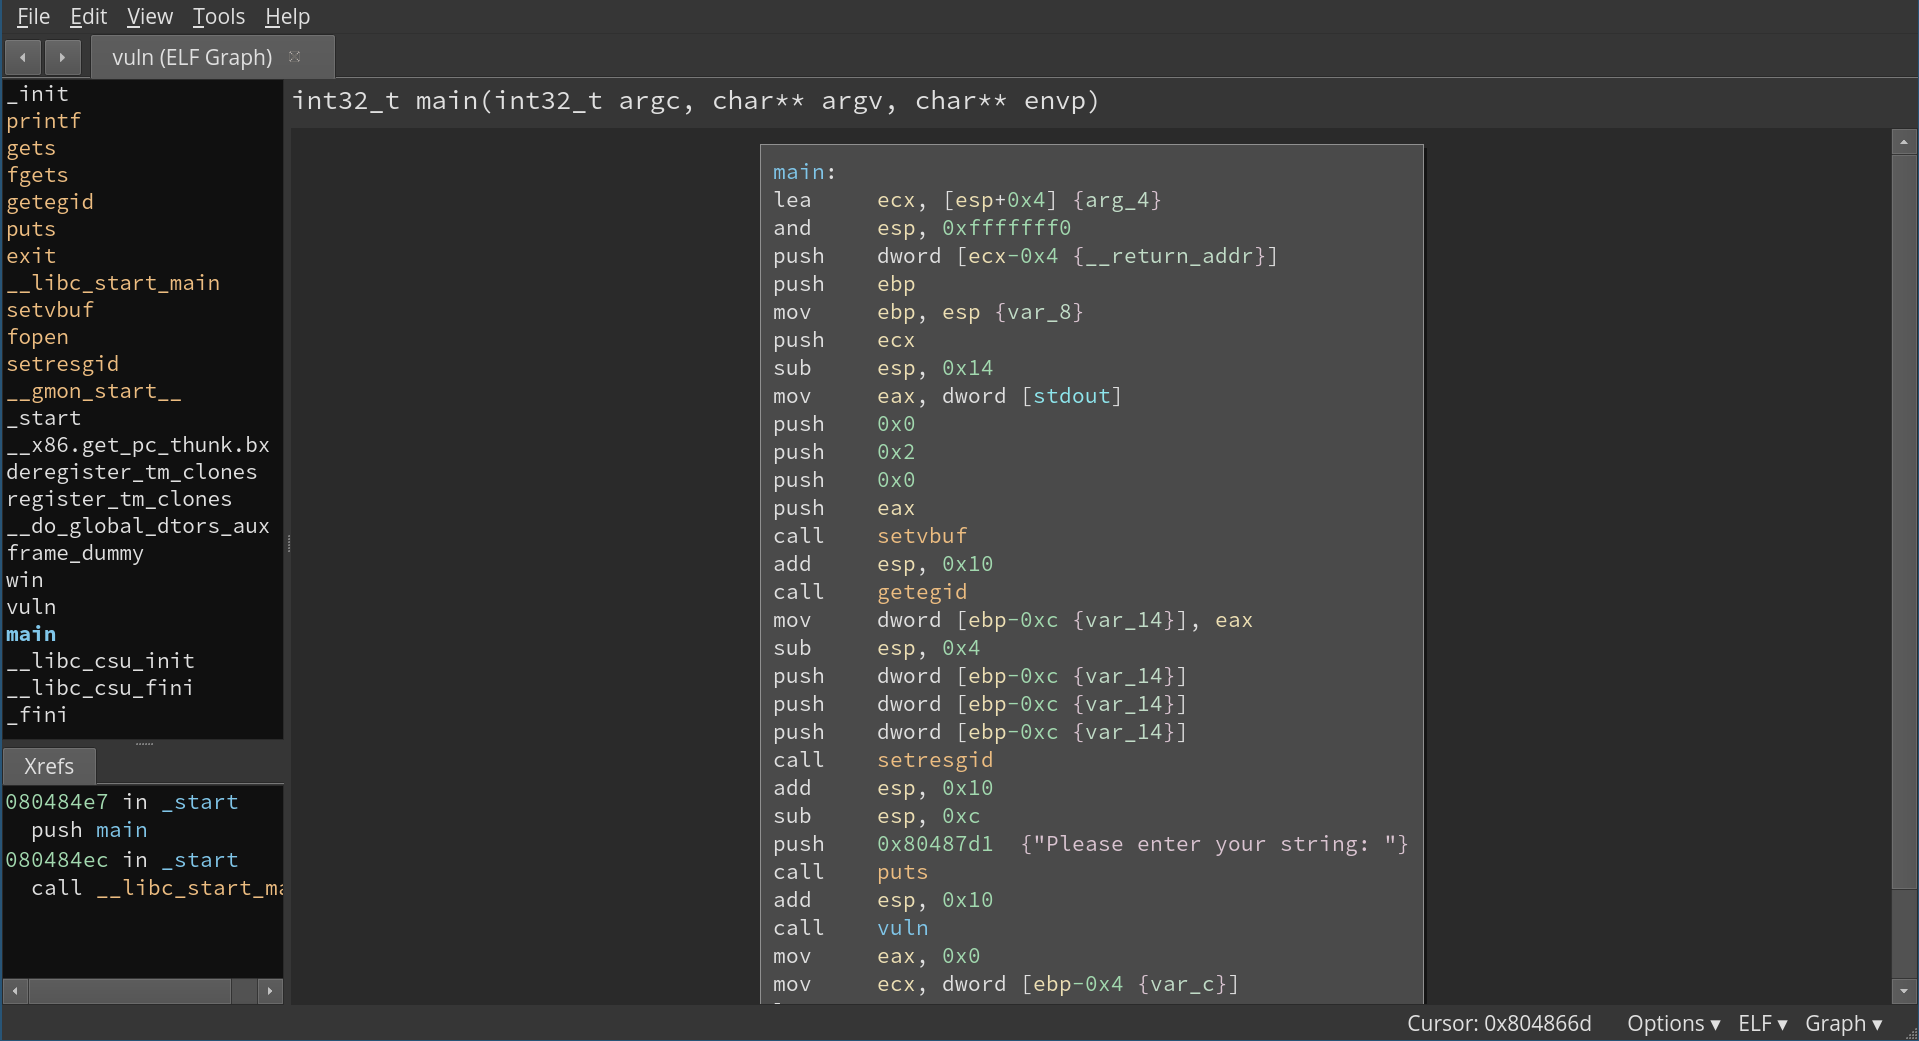
\includegraphics[width=1.2\textwidth]{BNinja1.png}}
    \centering
\end{figure}
Binary Ninja provides many features.  For one it is really nice to read outside of a terminal
window and it color codes things to make it more visually appealing.  You can double click on
variables to change their names to something more helpful.  There is a graph layout for the
assembly that at first looks similar to objdump but you will notice that it better shows the
flow of a function by displaying the branches apart from one another.  It is also very clear
and easy to see all the user functions and what functions are library/system functions.  There
is a lot of functionality in Binary Ninja that we have not even explored yet.  I would highly
suggest that you open it up one some program and just start looking around in it and look up
Binary Ninja plug-ins.  Binary Ninja has some other functions such as noping out a line or 
helping with unpacking a binary.  noping out some of the program is called Binary Patching. 
Binary Patching and unpacking a binary are both examples of defeating some anti-reversing 
techniques.
\begin{figure}[b]
	\hbox{\hspace{-5em} 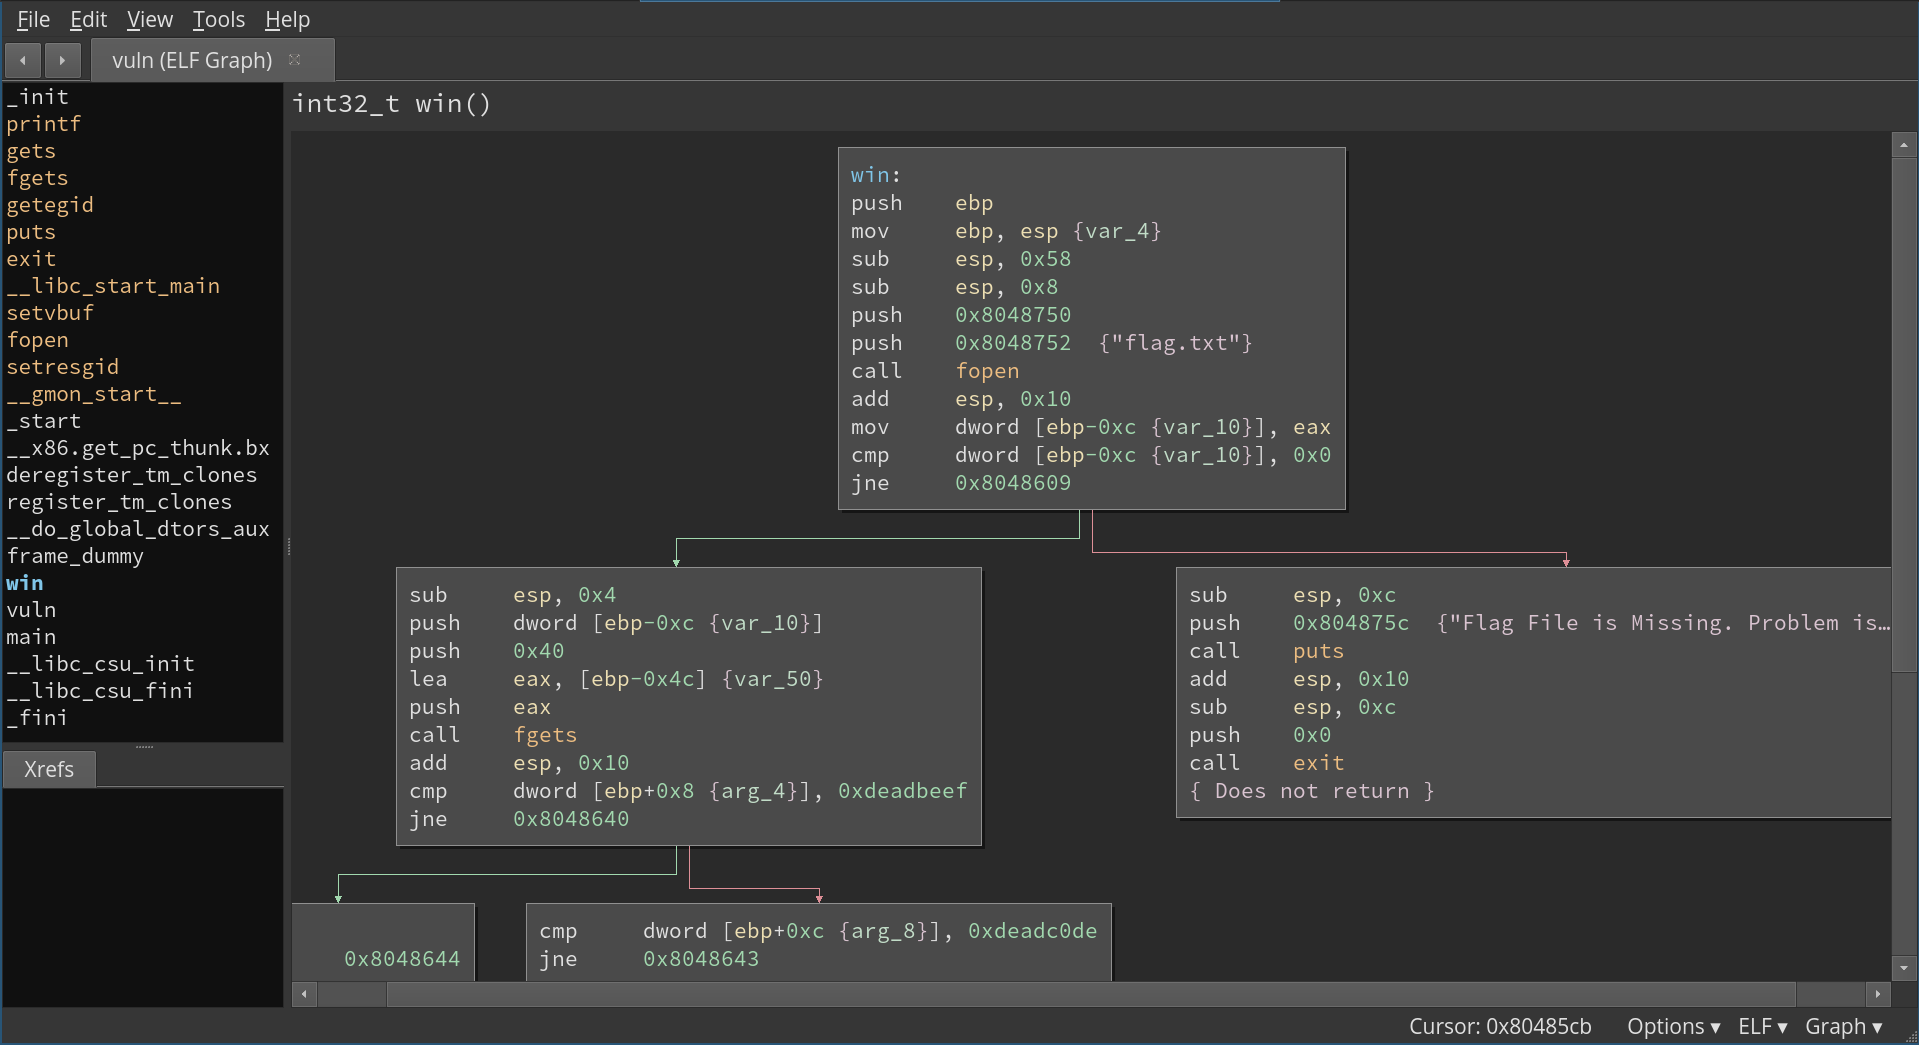
\includegraphics[width=1.2\textwidth]{BNinja2.png}}
    \centering
\end{figure}

\section{Ghidra}
Ghidra is a static analysis tool that can disassemble binaries similar to objdump, it can create a 
flow chart like Binary Ninja, and it can decompile binaries like IDA Pro hexrays.  And, it is free.
This makes Ghirda a game changer.  It is pretty easy to use as well.  Right when you open a program
up in it it will ask you if you want to analyse the program.  And when you do it will also decompile
everything into decently readable code.  So any function that you click on will display both
the disassembly as well as the decomplation right next to each other.


\chapter{Anti-Reversing Techniques and How to Get Around Them}
There are many techniques that people writing programs can use to make it much harder for a person to reverse engineer their program.  These techniques are often called anti-reversing.  We will cover a few of the most basic techniques and how to get around them.

\section{Stripped Binaries}
When a program gets compiled there is a option with the compiler to strip the binary.
What this means is that it takes away many of the debugging symbols in the program.
Therefore there is not longer any main in the compiled program or any other function
names for that matter.  They are not necessary for the program to run and therefore 
are stripped out of it.  All binaries start at \_start which then normally calls 
main.  But in the case of a stripped binary it \_start does the setup that it always 
does (just usually in the background) and makes some calls and eventually ends up 
running the code for the main function.

This is used to shrink down the size of the binary file and potentially give better
performance.  The only problem is that it makes it more difficult to reverse engineer because
there are no user created function names.

The key to reversing a stripped binary is to focus on the key instructions that you 
care about.  If you are given the source code then you can start out by using that
as a reference for what the x86 instructions are doing.  If you do not have the source
code then run the program a couple of times and start by thinking about what it is doing.
It will almost certain start off with printing out something whether it is a usage 
message, error message, or just a normal message.  Either way, if you have the source
or you don't, you can figure out what the first couple functions that the program calls
are.

With this information, you can figure out where the program actually starts.  So
open up objdump and search for the function that you think is the beginning of the program.
From here you can start reversing like normal following along the program trying to 
map out what each of the functions do.

NOTE: \url{https://reverseengineering.stackexchange.com/questions/1935/how-to-handle-stripped-binaries-with-gdb-no-source-no-symbols-and-gdb-only-sho}  Read this for extra instructions

\section{Binary Patching}
It is not uncommon (especially in CTFs) that you will find a program that makes a call to an unnecessary function whose purpose is simply to waste time.  Or perhaps it calls a function that sets a timer that kills the process after a few seconds.  This would mean that the program should have enough time to run normally but not enough time if someone ran it in something that pauses the program such as GDB.  Or even a program that kills itself and was never fully intended to be run at all.  Now there are a couple of different methods of getting around this type of anti-reversing.  We could merely tell GDB to step around said function by breaking right before the function call and then running the ``set'' command in GDB (set \$eip=0x08462a24) or whatever the instruction after the function call is.  We could even setup something at a break point such that when it breaks right before the call it does this command and then continues on normally.  But this isn't very elegant.  There has to be a better way...
Maybe some way we could patch the binary such that it did not have the bad function calls anymore...

What if we just deleted the bytes that called that function from the binary?  Well we should not actually delete bytes because that can be dangerous and mess up the stack alignment and therefore the program might not run properly.  But we could always convert them to nops.  This way there is just as many bytes in the program as before and the stack is still perfectly aligned.  In fact the purpose of the nop opcode in general is for stack alignment.  We know that the hexdump of the program is simply the instruction opcodes and so if we edit the hex of the program then we are editing the opcodes as well.  The best way to do this is to open up objdump and find the hex that we want to nop out.
\begin{lstlisting}
  400832:       48 89 75 f0             mov    QWORD PTR [rbp-0x10],rsi
  400836:       b8 00 00 00 00          mov    eax,0x0
  40083b:       e8 a9 ff ff ff          call   4007e9 <header>
  400840:       b8 00 00 00 00          mov    eax,0x0
  400845:       e8 f8 fe ff ff          call   400742 <set_timer>
  40084a:       b8 00 00 00 00          mov    eax,0x0
  40084f:       e8 42 ff ff ff          call   400796 <get_key>
\end{lstlisting}
In this example we have a program from picoCTF2018 be-quick-or-be-dead-1.  This problem sets a timer that kills the program after a very short period of time such that it cannot get the flag if it is run as is.  So we are gonna patch it such that it does not have this call to this timer anymore.  We see that we need to turn the opcodes ``e8 f8 fe ff ff'' into ``90 90 90 90 90''.  To do this we are gonna edit the hex of the program so we can run hexeditor on the program.  Hexeditor is a nano like hexeditor which works if you know how to use nano but I never use nano so I don't like it very much.
We generally use a program called hte \url{https://github.com/sebastianbiallas/ht} but either way search for the bytes that we need to change.  Edit them so that they are 90s instead and save and exit.  Now look back at the objdump and the call is gone and in it's place is a bunch of nops.
\begin{lstlisting}
  400832:       48 89 75 f0             mov    QWORD PTR [rbp-0x10],rsi
  400836:       b8 00 00 00 00          mov    eax,0x0
  40083b:       e8 a9 ff ff ff          call   4007e9 <header>
  400840:       b8 00 00 00 00          mov    eax,0x0
  400845:       90                      nop
  400846:       90                      nop
  400847:       90                      nop
  400848:       90                      nop
  400849:       90                      nop
  40084a:       b8 00 00 00 00          mov    eax,0x0
  40084f:       e8 42 ff ff ff          call   400796 <get_key>
\end{lstlisting}
Now you can run it just like that function was never even there.  Be careful not to remove any necessary functionality such as if the function you nop'ed out had a return value that gets checked (in that case you could just nop out the check too or you might have to do some more even janky-er patching where you put into eax the value that it would need).

This same thing can be also done in Binary Ninja.


\section{Packing and unpacking}
Packing is a technique that a program can use where they will change the .text segment on the file as the program is being executed.  This is to make static analysis more difficult.  One of the most common method of this is to xor all the bytes of a given area with some value.  Then when you go to objdump the binary it largely looks like garbage.  

\begin{lstlisting}
0804842b <auth>:
 804842b:       55                      push   ebp
 804842c:       89 e5                   mov    ebp,esp
 804842e:       81 ec 98 00 00 00       sub    esp,0x98
 8048434:       a1 fc 91 04 08          mov    eax,ds:0x80491fc
 8048439:       83 f8 ff                cmp    eax,0xffffffff
 804843c:       74 4c                   je     804848a <start_452>
 804843e:       c7 05 fc 91 04 08 01    mov    DWORD PTR ds:0x80491fc,0x1
 8048445:       00 00 00 
 8048448:       8d 05 8a 84 04 08       lea    eax,ds:0x804848a
 804844e:       a3 f4 91 04 08          mov    ds:0x80491f4,eax
 8048453:       a1 f4 91 04 08          mov    eax,ds:0x80491f4
 8048458:       25 00 f0 ff ff          and    eax,0xfffff000
 804845d:       83 ec 04                sub    esp,0x4
 8048460:       6a 07                   push   0x7
 8048462:       68 00 20 00 00          push   0x2000
 8048467:       50                      push   eax
 8048468:       e8 83 fe ff ff          call   80482f0 <mprotect@plt>
 804846d:       83 c4 10                add    esp,0x10
 8048470:       8d 05 8a 84 04 08       lea    eax,ds:0x804848a

08048476 <repeat_452>:
 8048476:       81 38 9b 1b 18 25       cmp    DWORD PTR [eax],0x25181b9b
 804847c:       74 0c                   je     804848a <start_452>
 804847e:       66 81 30 73 61          xor    WORD PTR [eax],0x6173
 8048483:       40                      inc    eax
 8048484:       eb f0                   jmp    8048476 <repeat_452>
 8048486:       9b                      fwait
 8048487:       1b 18                   sbb    ebx,DWORD PTR [eax]
 8048489:       25                      .byte 0x25

0804848a <start_452>:
 804848a:       b4 97                   mov    ah,0x97
 804848c:       66 ed                   in     ax,dx
 804848e:       ed                      in     eax,dx
 804848f:       ed                      in     eax,dx
 8048490:       13 12                   adc    edx,DWORD PTR [edx]
\end{lstlisting}

This program has been packed.  It is not exactly easy to tell right away but if you look at it, the instructions seem weird.  The last instruction of repeat\_452 is ``.byte 0x25'' which is not even an instruction.  It is merely saying that the byte 25 is there but there is not instruction that matches that.  This is not something that you will see in an ordinary binary.  The more you look at this especially down in the start\_452 it begins to look weirder and weirder.  There is an fwait?  ssb?  what is the in instruction?  adc?  I have never seen most of these commands. 

So we know that it is packed.  Can we not run this program?  This program calls auth which executes down to its end and then starts executing repeat\_452, which isn't actually a function.  repeat\_452 is a loop that start with eax pointing to the dereferenced pointer 0x804848a which is the start\_452 label.  From there it xors four bytes at a time with 0x25181b9b.  This continues down the .text until the end.  Then it is able to continue through and execute this unpacked file.  

We can do the unpacking ourselves and then do some static analysis on it.  This is a pretty simple program that doesn't require much analysis once we unpack it so we can simply run it in gdb and break after it is finished running it's unpacking function and then disass it.  However, this method may not work in other programs so we are going to learn how to unpack binaries using binary ninja.

\subsection{Example Problems}
Hackcenter Cyberstakes 2015: packing, multi-packing


\chapter{Writing assembly}
Writing assembly is not as complicated as it may seem.  If you know enough to be able to read assembly then you know enough to be able to write it.  An assembly file generally ends with a .asm and more or less looks like an objdump without all the stuff to the left of the instructions.

\section{sections}
If we think back to the memory structure when a binary gets loaded there are multiple sections.  The reserved, stack, heap, text, data, and bss sections.  Well we know that the stack and heap are used during the program execution but the text section which holds the program instructions as well as the bss and data which holds global data are created at compilation time.  When we are writing the assembly ourselves we need to write the .text, data, and bss sections as they are needed.  Let's look go back to the assembly and c side by side but this time let's look at a simple hello world program.

\begin{minipage}{.45\textwidth}
\begin{lstlisting}[caption=c hello world,frame=tlrb]{Control Flow}
#include <stdio.h>
int main(){
	char message[] = "Hello World!\n";
	printf(hello);
	return 0;
}
\end{lstlisting}
\end{minipage}\hfill
\begin{minipage}{.45\textwidth}
\begin{lstlisting}[caption=assembly 32bit,frame=tlrb]{Control Flow 32}
extern printf
extern exit

section .text
global _start

_start:
      push message
      call printf
      add esp,0x4

      push 0x0
      call exit

section .data
      message db "Hello World!", 0xa, 0x00

\end{lstlisting}
\end{minipage}

Here you can see that we wrote the data section and .text sections ourselves we did not write any bss section as it was not needed for this.  In the data section we declare the global variables that we are going to use in this program which in this case is the Hello World string.  Then in the .text section we have to write the instructions.  All programs start with the \_start function this is the program that usually sets everything up and then calls main.  We declare this function as global so that the compiler knows where it is. Just as we would see in the objdump, we need to push all the arguments to each function onto the stack in reverse order before we call them.  In the c program we had to specify where printf was we have to tell our assembly program that it is declared outside of this program and we do this with $extern$.  Hopfully this isn't too large a jump from reading x86.   

\section{Compilation}
The next question that we come to is how do we compile a .asm file?  We cannot simply use gcc like we would a c file, can we? No.  It's slightly more complicated.  There is a program call nasm that can be used to assemble assembly instructions into object files.  This basically means that it will assembly our instructions but they are not actually in a executable format yet.  We can use nasm like: |nasm -f elf32 -o hello.o hello.asm|.  The -f elf32 option tells nasm that we are assembling our program into an elf (executable and linking format) of 32 bits.  

The next process is to turn our object file (.o) into an executable file.  We can do that with ld (the GNU Linker).  "ld combines a number of object and archive files, relocates their data and ties up symbol references.  Usually the last step in compiling a program is to run ld." - ld man page.  We have a couple of symbol references in our code.  The message for one is a reference as well as our \_start.  These are local references but they are references none the less and the compiled binary needs to know where these things are.  We also have two external functions that we are calling (printf and exit) which need to be properly referenced.  In this case we need to run: |ld -m elf_i386 test.o -o test -lc --dynamic-linker /lib32/ld-2.27.so|.  The -m once again tells the computer that it needs to be a 32 bit elf binary.  The -lc we need to use because we called printf and need to link to it's code which the 32 bit version is in /lib32/ld-2.27.so with the --dynamic-linker to tell the compiler to link dynamically instead of statically.


\chapter{Reversing Windows Binaries}

\chapter{Other Assembly Languages}
There are many different assembly languages.  If you are a CS major then you have (or will) learn mips, if you're cyber then you learned some other weird thing.  Learning multiple assembly languages creates a depth of understanding and takes it easier to read assembly in general and to transition to a language that you have never seen before.  x86 assembly language is the most common on most desktop/laptop computers and therefore the one that we teach.  There are, however, many more assembly languages out there some of which it could be beneficial to learn. ARM is a popular one these days.  It is on most phones and IoT devices.  If you're gonna be learning to hack either of these systems then I would encourage learning ARM.  

\end{document}
